
\chapter{Introduction}\label{chapter:introduction}
%Breast cancer bad 
Breast cancer is the most common form of cancer diagnosed worldwide
and the leading cause of cancer-related death among women.~\cite{chhikara2022global}
It is a heterogeneous disease, consisting of several morphological and molecular subtypes.
The molecular subtypes are among the most important factors to characterize
breast cancer. Four main groups are defined
based on the status of several receptors used in clinical practice~\cite{home},
namely the Hormonal Receptor (HR, which is positive if either Estrogen Receptor (ER) or Progesterone Receptor (PR) are positive)
and of their human epidermal growth factor receptor 2 (Her2):
\begin{enumerate}
    \itemsep0em 
    \item Luminal A (HR positive, Her2 negative)
    \item Luminal B (HR positive, Her2 positive)
    \item Her2 enriched (HR negative, Her2 positive) 
    \item Triple Negative (HR negative, Her2 negative)
\end{enumerate}
Regardless of the subtype, for diagnostic confirmation of breast cancer
a patient’s tissue sample is sectioned
onto microscope slides for staining, often with hematoxylin and eosin (H\&E), followed by
a visual diagnosis by a pathologist. Pathologists examine a tissue specimen
for abnormalities that indicate breast cancer. 
Since cancer causes changes in tissue at the sub-cellular scale, an analysis of normal and tumor tissue can provide novel insights into
tissue characteristics and can lead to a better understanding of mechanisms underlying cancer onset, progression
and provide valuable information for medical decision making such as treatment choices.~\cite{vu2019methods}
While the manual examination continues to be widely applied in clinical settings, it is a
subjective and is not scalable to translational and clinical research studies
involving a high number of high-resolution whole slide tissue images (WSIs). 
Hence, there is an increased need
for reliable and efficient automated methods to complement the traditional manual
examination of tissue samples. 
Due to advancing technology and access to a large amount of data, deep learning methods
have garnered a lot of interest in computer vision for the digital pathology domain.
The two most common computerized tasks in WSI
analysis are the segmentation of microscopic structures, structures like tumor regions and
smaller nuclei and cells, and the classification of image regions or even whole images.
And while there are a great number of deep learning based analysis pipelines in the digital pathology domain,
automated algorithms also contribute to the development and testing of reliable prognostic and predictive biomarkers
to help clinicians choose the best treatment for each patient.

The differentiation between breast cancer
types and subtypes is essential. This thesis is focused on Her2 positive
and Triple Negative breast cancer (TNBC) subtypes since they have the worst prognosis,
and therefore subject to a large corpus of research in prognostic and predictive biomarkers,
aiming at improving patient management and prognosis. TNBC is an aggressive type of cancer and
due to the lack of all three receptors, it has a limited response to hormonal and immune treatments.
Cancers of this type are known to have high recurrence rates and
poor prognoses compared to non-TN breast cancers.~\cite{cao2020triple}
There are multiple reported biomarkers for TNBC, such as epidermal growth factor receptor,
vascular endothelial growth factor, C-kit, and basal cytokeratins.~\cite{yadav2015biomarkers} Moreover, a significant
percentage of TNBCs are known to carry BRCA1 mutations,
in which tumor cells are defective in homologous recombination DNA repair mechanisms.
But this thesis focuses on the tumor-infiltrating lymphocytes (TILs), which could be examined 
from WSIs therefore directly accessible without the need for any further testing or additional data source. 

TILs are mononuclear immune cells that infiltrate tumor tissue and have been detected in almost all solid tumors,
including breast cancer.~\cite{laenkholm2022incorporation}
The development and progression of malignant tumors can be characterized by an interaction of the cells
in the tumor microenvironment and TILs.
In the early stage HER2-positive and TNBC, immune infiltrates are detectable in up to 75\% of tumors.~\cite{dieci2018update}
Accumulating evidence indicates that tumor-infiltrating lymphocytes are clinically useful biomarkers in TNBC and HER2-positive
and that they play an essential role in cancer progression.~\cite{gao2020prognostic}
The patients with a high proportion of TILs in the tumor tissue and high immunogenicity of the tumor
were shown to respond better to the chemotherapy. Further research and development of additional
TILs related biomarkers would not only grand clinicians important prognostic information but also promote the
research focus of novel treatments and therapeutics.
Analysis of TILs with exhausted phenotype is associated with loss of antitumor immunity.
Single-cell RNA-seq of TILs has been already performed to search for new immune checkpoint blockade targets that enable
the precise definition and even novel development of therapeutic strategies to overcome T-cell exhaustion.
Therapeutic approaches to influence T-cell exhaustion have been already developed to target proteins CTLA-4, PD-1, and PD-L1
and have proven to be effective in treating melanoma and non-small-cell lung cancer during ongoing trials.~\cite{postow2015immune}
TILs in TNBC patients also display immuno-suppressive phenotypes~\cite{chung2017single} and the number of TILs detected by TNBC
patients is higher than in other breast cancer subgroups~\cite{schneeweiss2019diagnosis} which makes TNBC a valid target for further
TILs sequencing research for its application in the context of TN breast cancer or in search of further targets.

The aim of this work is to experiment with computer algorithms for the automated image segmentation and tumor-infiltrating
lymphocytes assessment in Her2 positive
and Triple Negative breast cancer histopathology slides based on Tumor InfiltratinG lymphocytes in
breast cancER (TiGER) challenge. This works partly relies on publically
released TiGER challenge and TCGA dataset to also further experiment with the prognostic significance of computer-generated TILs scores
for predicting patients' survival based on combined cell- and tissue-level information of WSIs. 

\begin{figure}
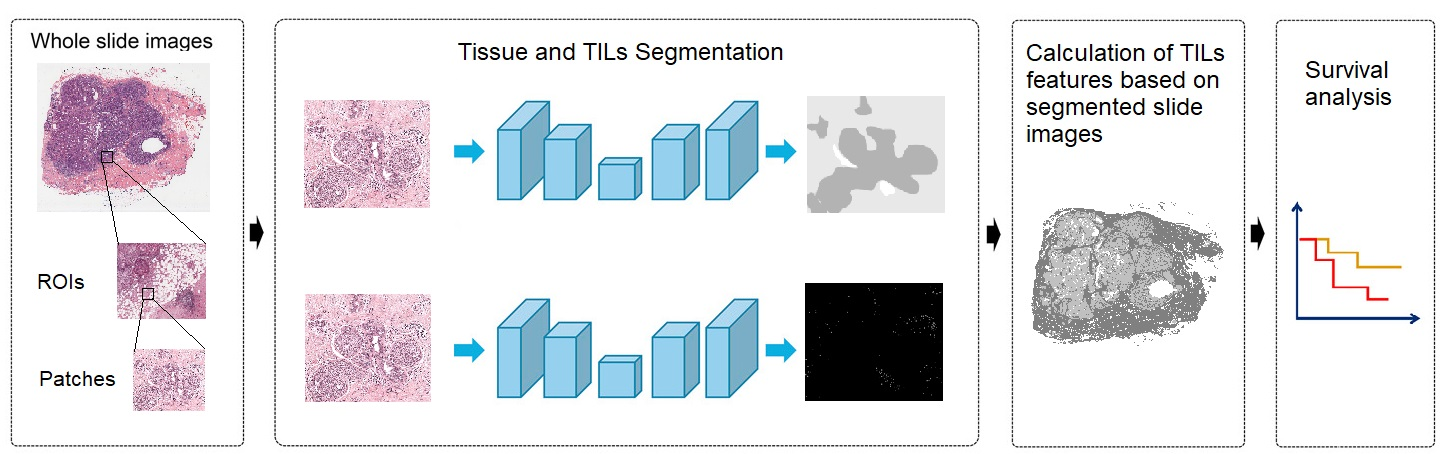
\includegraphics[width=\linewidth]{figures/overview.jpg}
\caption{EXAMPLES for TILs prediction models. A lot of test comming up here.}
\label{fig:figure3}
\end{figure}

